% Options for packages loaded elsewhere
\PassOptionsToPackage{unicode}{hyperref}
\PassOptionsToPackage{hyphens}{url}
%
\documentclass[
]{article}
\usepackage{amsmath,amssymb}
\usepackage{iftex}
\ifPDFTeX
  \usepackage[T1]{fontenc}
  \usepackage[utf8]{inputenc}
  \usepackage{textcomp} % provide euro and other symbols
\else % if luatex or xetex
  \usepackage{unicode-math} % this also loads fontspec
  \defaultfontfeatures{Scale=MatchLowercase}
  \defaultfontfeatures[\rmfamily]{Ligatures=TeX,Scale=1}
\fi
\usepackage{lmodern}
\ifPDFTeX\else
  % xetex/luatex font selection
\fi
% Use upquote if available, for straight quotes in verbatim environments
\IfFileExists{upquote.sty}{\usepackage{upquote}}{}
\IfFileExists{microtype.sty}{% use microtype if available
  \usepackage[]{microtype}
  \UseMicrotypeSet[protrusion]{basicmath} % disable protrusion for tt fonts
}{}
\makeatletter
\@ifundefined{KOMAClassName}{% if non-KOMA class
  \IfFileExists{parskip.sty}{%
    \usepackage{parskip}
  }{% else
    \setlength{\parindent}{0pt}
    \setlength{\parskip}{6pt plus 2pt minus 1pt}}
}{% if KOMA class
  \KOMAoptions{parskip=half}}
\makeatother
\usepackage{xcolor}
\usepackage[margin=1in]{geometry}
\usepackage{graphicx}
\makeatletter
\def\maxwidth{\ifdim\Gin@nat@width>\linewidth\linewidth\else\Gin@nat@width\fi}
\def\maxheight{\ifdim\Gin@nat@height>\textheight\textheight\else\Gin@nat@height\fi}
\makeatother
% Scale images if necessary, so that they will not overflow the page
% margins by default, and it is still possible to overwrite the defaults
% using explicit options in \includegraphics[width, height, ...]{}
\setkeys{Gin}{width=\maxwidth,height=\maxheight,keepaspectratio}
% Set default figure placement to htbp
\makeatletter
\def\fps@figure{htbp}
\makeatother
\setlength{\emergencystretch}{3em} % prevent overfull lines
\providecommand{\tightlist}{%
  \setlength{\itemsep}{0pt}\setlength{\parskip}{0pt}}
\setcounter{secnumdepth}{-\maxdimen} % remove section numbering
\usepackage{booktabs}
\usepackage{longtable}
\usepackage{array}
\usepackage{multirow}
\usepackage{wrapfig}
\usepackage{float}
\usepackage{colortbl}
\usepackage{pdflscape}
\usepackage{tabu}
\usepackage{threeparttable}
\usepackage{threeparttablex}
\usepackage[normalem]{ulem}
\usepackage{makecell}
\usepackage{xcolor}
\ifLuaTeX
  \usepackage{selnolig}  % disable illegal ligatures
\fi
\usepackage{bookmark}
\IfFileExists{xurl.sty}{\usepackage{xurl}}{} % add URL line breaks if available
\urlstyle{same}
\hypersetup{
  pdftitle={Randomized Experiment},
  hidelinks,
  pdfcreator={LaTeX via pandoc}}

\title{Randomized Experiment}
\author{}
\date{\vspace{-2.5em}}

\begin{document}
\maketitle

\section{Analyze attack trends}\label{analyze-attack-trends}

\begin{figure}[tb]

{\centering 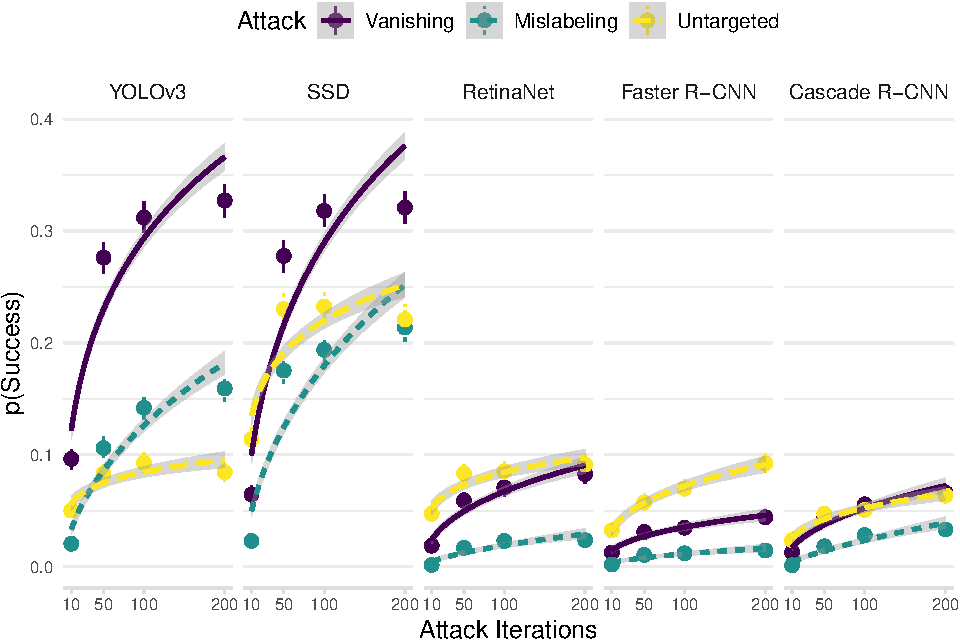
\includegraphics[width=1\linewidth]{imgs/success_trend_graph-1} 

}

\caption{Intent obfuscating attack is feasible for all models and attacks:  We conduct a randomized experiment by resampling COCO images, and within those images randomly sampling correctly predicted target and perturb objects. Then we distort the perturb objects to disrupt the target objects varying the attack iterations. The binned summaries and regression trendlines graph success proportion against attack iterations in the randomized attack experiment. Errors are 95\% confidence intervals and every point aggregates success over 4,000 images. Targeted vanishing and mislabeling attacks obtain significantly greater success on the 1-stage YOLOv3 and SSD than the 2-stage Faster R-CNN and Cascade R-CNN detectors. However, the 1-stage RetinaNet is as resilient as the 2-stage detectors. Moreover, success rates significantly increase with larger attack iterations. Significance is determined at $\alpha < 0.05$ using a Wald z-test on the logistic estimates. Full details are given in Section \ref{sec:rand_att}.}\label{fig:success_trend_graph}
\end{figure}

\begingroup\fontsize{9}{11}\selectfont

\begin{longtable}[t]{lllrrrrrr}
\caption{\label{tab:model_stage_table}We run a logistic model regressing success against detection models, split by attack, in the randomized attack experiment. Both vanishing and mislabeling attacks obtain higher success on 1-stage (YOLOv3, SSD) than 2-stage (Faster R-CNN, Cascade R-CNN) detectors. However, the 1-stage RetinaNet is as resilient as 2-stage detectors. Table headers are explained in Appendix \ref{app:tab_hdr}.}\\
\toprule
\multicolumn{1}{c}{Group} & \multicolumn{8}{c}{Regression} \\
\cmidrule(l{3pt}r{3pt}){1-1} \cmidrule(l{3pt}r{3pt}){2-9}
Attack & term & sig & estimate & std.error & statistic & p.value & conf.low & conf.high\\
\midrule
 & YOLOv3 &  & 0.000 &  &  &  &  & \\
\cmidrule{2-9}\nopagebreak
 & SSD &  & -0.029 & 0.048 & -0.597 & 0.550 & -0.122 & 0.065\\
\cmidrule{2-9}\nopagebreak
 & RetinaNet & * & -1.685 & 0.067 & -25.317 & 0.000 & -1.817 & -1.556\\
\cmidrule{2-9}\nopagebreak
 & Faster R-CNN & * & -2.352 & 0.084 & -28.021 & 0.000 & -2.519 & -2.190\\
\cmidrule{2-9}\nopagebreak
\multirow{-5}{*}{\raggedright\arraybackslash Vanishing} & Cascade R-CNN & * & -1.929 & 0.072 & -26.776 & 0.000 & -2.072 & -1.790\\
\cmidrule{1-9}\pagebreak[0]
 & YOLOv3 &  & 0.000 &  &  &  &  & \\
\cmidrule{2-9}\nopagebreak
 & SSD & * & 0.361 & 0.058 & 6.239 & 0.000 & 0.248 & 0.475\\
\cmidrule{2-9}\nopagebreak
 & RetinaNet & * & -2.052 & 0.112 & -18.248 & 0.000 & -2.278 & -1.837\\
\cmidrule{2-9}\nopagebreak
 & Faster R-CNN & * & -2.555 & 0.139 & -18.371 & 0.000 & -2.838 & -2.292\\
\cmidrule{2-9}\nopagebreak
\multirow{-5}{*}{\raggedright\arraybackslash Mislabeling} & Cascade R-CNN & * & -1.706 & 0.098 & -17.372 & 0.000 & -1.902 & -1.517\\
\cmidrule{1-9}\pagebreak[0]
 & YOLOv3 &  & 0.000 &  &  &  &  & \\
\cmidrule{2-9}\nopagebreak
 & SSD & * & 1.123 & 0.068 & 16.407 & 0.000 & 0.990 & 1.258\\
\cmidrule{2-9}\nopagebreak
 & RetinaNet &  & 0.084 & 0.079 & 1.066 & 0.286 & -0.071 & 0.239\\
\cmidrule{2-9}\nopagebreak
 & Faster R-CNN &  & 0.099 & 0.079 & 1.259 & 0.208 & -0.055 & 0.254\\
\cmidrule{2-9}\nopagebreak
\multirow{-5}{*}{\raggedright\arraybackslash Untargeted} & Cascade R-CNN & * & -0.304 & 0.086 & -3.531 & 0.000 & -0.474 & -0.136\\
\bottomrule
\end{longtable}
\endgroup{}

\begingroup\fontsize{9}{11}\selectfont

\begin{longtable}[t]{lllrrrrrr}
\caption{\label{tab:target_untarget_vanish_mislabel_table}We run a logistic model regressing success against attacks, split by detection models in the randomized attack experiment. Targeted attacks obtain higher success than untargeted attacks on YOLOv3 and SSD. Within targeted attacks, vanishing attacks obtain higher success than mislabeling attacks on all models. Table headers are explained in Appendix \ref{app:tab_hdr}.}\\
\toprule
\multicolumn{1}{c}{Group} & \multicolumn{8}{c}{Regression} \\
\cmidrule(l{3pt}r{3pt}){1-1} \cmidrule(l{3pt}r{3pt}){2-9}
Model & term & sig & estimate & std.error & statistic & p.value & conf.low & conf.high\\
\midrule
 & Vanishing &  & 0.000 &  &  &  &  & \\
\cmidrule{2-9}\nopagebreak
 & Mislabeling & * & -0.943 & 0.055 & -17.212 & 0.000 & -1.051 & -0.836\\
\cmidrule{2-9}\nopagebreak
\multirow{-3}{*}{\raggedright\arraybackslash YOLOv3} & Untargeted & * & -1.662 & 0.066 & -25.151 & 0.000 & -1.793 & -1.534\\
\cmidrule{1-9}\pagebreak[0]
 & Vanishing &  & 0.000 &  &  &  &  & \\
\cmidrule{2-9}\nopagebreak
 & Mislabeling & * & -0.553 & 0.051 & -10.779 & 0.000 & -0.654 & -0.453\\
\cmidrule{2-9}\nopagebreak
\multirow{-3}{*}{\raggedright\arraybackslash SSD} & Untargeted & * & -0.511 & 0.051 & -10.017 & 0.000 & -0.611 & -0.411\\
\cmidrule{1-9}\pagebreak[0]
 & Vanishing &  & 0.000 &  &  &  &  & \\
\cmidrule{2-9}\nopagebreak
 & Mislabeling & * & -1.311 & 0.119 & -11.047 & 0.000 & -1.548 & -1.082\\
\cmidrule{2-9}\nopagebreak
\multirow{-3}{*}{\raggedright\arraybackslash RetinaNet} & Untargeted &  & 0.107 & 0.079 & 1.348 & 0.178 & -0.048 & 0.263\\
\cmidrule{1-9}\pagebreak[0]
 & Vanishing &  & 0.000 &  &  &  &  & \\
\cmidrule{2-9}\nopagebreak
 & Mislabeling & * & -1.146 & 0.153 & -7.493 & 0.000 & -1.454 & -0.853\\
\cmidrule{2-9}\nopagebreak
\multirow{-3}{*}{\raggedright\arraybackslash Faster R-CNN} & Untargeted & * & 0.789 & 0.094 & 8.370 & 0.000 & 0.606 & 0.976\\
\cmidrule{1-9}\pagebreak[0]
 & Vanishing &  & 0.000 &  &  &  &  & \\
\cmidrule{2-9}\nopagebreak
 & Mislabeling & * & -0.720 & 0.109 & -6.619 & 0.000 & -0.936 & -0.509\\
\cmidrule{2-9}\nopagebreak
\multirow{-3}{*}{\raggedright\arraybackslash Cascade R-CNN} & Untargeted &  & -0.037 & 0.091 & -0.409 & 0.683 & -0.215 & 0.141\\
\bottomrule
\end{longtable}
\endgroup{}

\begingroup\fontsize{9}{11}\selectfont

\begin{longtable}[t]{llllrrrrrr}
\caption{\label{tab:num_iteration_table}We run a logistic model regressing success against log(attack iterations) in the randomized attack experiment. Success rates increase with attack iterations for all models and attacks. Table headers are explained in Appendix \ref{app:tab_hdr}.}\\
\toprule
\multicolumn{2}{c}{Group} & \multicolumn{8}{c}{Regression} \\
\cmidrule(l{3pt}r{3pt}){1-2} \cmidrule(l{3pt}r{3pt}){3-10}
 & Attack & term & sig & estimate & std.error & statistic & p.value & conf.low & conf.high\\
\midrule
\addlinespace[0.3em]
\multicolumn{10}{l}{\textbf{YOLOv3}}\\
\hspace{1em} & Vanishing & log(iterations) & * & 0.476 & 0.019 & 25.267 & 0 & 0.439 & 0.513\\
\cmidrule{2-10}\nopagebreak
\hspace{1em} & Mislabeling & log(iterations) & * & 0.622 & 0.030 & 20.761 & 0 & 0.564 & 0.681\\
\cmidrule{2-10}\nopagebreak
\hspace{1em} & Untargeted & log(iterations) & * & 0.192 & 0.028 & 6.776 & 0 & 0.137 & 0.247\\
\cmidrule{1-10}\pagebreak[0]
\addlinespace[0.3em]
\multicolumn{10}{l}{\textbf{SSD}}\\
\hspace{1em} & Vanishing & log(iterations) & * & 0.566 & 0.020 & 28.456 & 0 & 0.527 & 0.605\\
\cmidrule{2-10}\nopagebreak
\hspace{1em} & Mislabeling & log(iterations) & * & 0.621 & 0.025 & 24.466 & 0 & 0.572 & 0.672\\
\cmidrule{2-10}\nopagebreak
\hspace{1em} & Untargeted & log(iterations) & * & 0.256 & 0.019 & 13.449 & 0 & 0.219 & 0.294\\
\cmidrule{1-10}\pagebreak[0]
\addlinespace[0.3em]
\multicolumn{10}{l}{\textbf{RetinaNet}}\\
\hspace{1em} & Vanishing & log(iterations) & * & 0.467 & 0.037 & 12.620 & 0 & 0.396 & 0.541\\
\cmidrule{2-10}\nopagebreak
\hspace{1em} & Mislabeling & log(iterations) & * & 0.635 & 0.076 & 8.331 & 0 & 0.490 & 0.789\\
\cmidrule{2-10}\nopagebreak
\hspace{1em} & Untargeted & log(iterations) & * & 0.225 & 0.029 & 7.802 & 0 & 0.169 & 0.282\\
\cmidrule{1-10}\pagebreak[0]
\addlinespace[0.3em]
\multicolumn{10}{l}{\textbf{Faster R-CNN}}\\
\hspace{1em} & Vanishing & log(iterations) & * & 0.397 & 0.049 & 8.160 & 0 & 0.303 & 0.494\\
\cmidrule{2-10}\nopagebreak
\hspace{1em} & Mislabeling & log(iterations) & * & 0.534 & 0.093 & 5.762 & 0 & 0.358 & 0.722\\
\cmidrule{2-10}\nopagebreak
\hspace{1em} & Untargeted & log(iterations) & * & 0.367 & 0.034 & 10.897 & 0 & 0.302 & 0.434\\
\cmidrule{1-10}\pagebreak[0]
\addlinespace[0.3em]
\multicolumn{10}{l}{\textbf{Cascade R-CNN}}\\
\hspace{1em} & Vanishing & log(iterations) & * & 0.502 & 0.043 & 11.736 & 0 & 0.419 & 0.587\\
\cmidrule{2-10}\nopagebreak
\hspace{1em} & Mislabeling & log(iterations) & * & 0.753 & 0.073 & 10.276 & 0 & 0.613 & 0.901\\
\cmidrule{2-10}\nopagebreak
\hspace{1em} & Untargeted & log(iterations) & * & 0.325 & 0.038 & 8.477 & 0 & 0.251 & 0.401\\
\bottomrule
\end{longtable}
\endgroup{}

\section{Analyze individual cases}\label{analyze-individual-cases}

\begin{figure}[tb]

{\centering 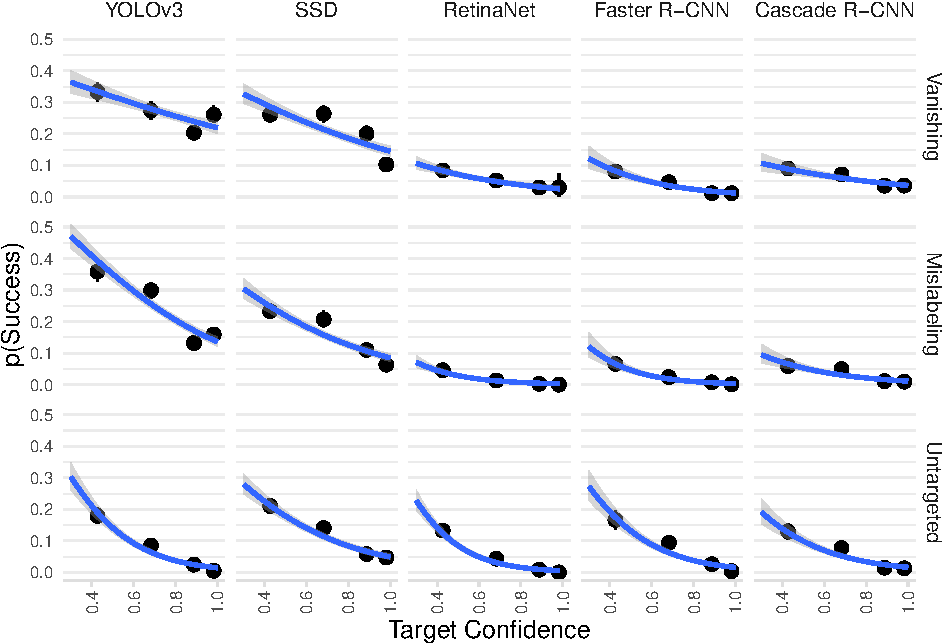
\includegraphics{imgs/target_conf_graph-1} 

}

\caption{Lower target confidence significantly increases success rates for all models and attacks:  The binned summaries and regression trendlines graph success proportion against target confidence in the randomized attack experiment. Bins are split into quantiles. Errors are 95\% confidence intervals}\label{fig:target_conf_graph}
\end{figure}

\begingroup\fontsize{9}{11}\selectfont

\begin{longtable}[t]{llllrrrrrr}
\caption{\label{tab:target_conf_table}We run a logistic model regressing success against target confidence in the randomized attack experiment. Lower target confidence significantly increases success rates for all models and attacks. Table headers are explained in Appendix \ref{app:tab_hdr}.}\\
\toprule
\multicolumn{2}{c}{Group} & \multicolumn{8}{c}{Regression} \\
\cmidrule(l{3pt}r{3pt}){1-2} \cmidrule(l{3pt}r{3pt}){3-10}
 & Attack & term & sig & estimate & std.error & statistic & p.value & conf.low & conf.high\\
\midrule
\addlinespace[0.3em]
\multicolumn{10}{l}{\textbf{YOLOv3}}\\
\hspace{1em} & Vanishing & confidence & * & -0.773 & 0.153 & -5.059 & 0 & -1.072 & -0.473\\
\cmidrule{2-10}\nopagebreak
\hspace{1em} & Mislabeling & confidence & * & -2.230 & 0.160 & -13.915 & 0 & -2.545 & -1.917\\
\cmidrule{2-10}\nopagebreak
\hspace{1em} & Untargeted & confidence & * & -3.910 & 0.268 & -14.579 & 0 & -4.442 & -3.390\\
\cmidrule{1-10}\pagebreak[0]
\addlinespace[0.3em]
\multicolumn{10}{l}{\textbf{SSD}}\\
\hspace{1em} & Vanishing & confidence & * & -1.063 & 0.142 & -7.505 & 0 & -1.341 & -0.786\\
\cmidrule{2-10}\nopagebreak
\hspace{1em} & Mislabeling & confidence & * & -1.616 & 0.151 & -10.714 & 0 & -1.913 & -1.321\\
\cmidrule{2-10}\nopagebreak
\hspace{1em} & Untargeted & confidence & * & -2.326 & 0.164 & -14.203 & 0 & -2.649 & -2.007\\
\cmidrule{1-10}\pagebreak[0]
\addlinespace[0.3em]
\multicolumn{10}{l}{\textbf{RetinaNet}}\\
\hspace{1em} & Vanishing & confidence & * & -3.057 & 0.321 & -9.535 & 0 & -3.695 & -2.437\\
\cmidrule{2-10}\nopagebreak
\hspace{1em} & Mislabeling & confidence & * & -6.133 & 0.616 & -9.952 & 0 & -7.389 & -4.969\\
\cmidrule{2-10}\nopagebreak
\hspace{1em} & Untargeted & confidence & * & -6.050 & 0.400 & -15.130 & 0 & -6.853 & -5.284\\
\cmidrule{1-10}\pagebreak[0]
\addlinespace[0.3em]
\multicolumn{10}{l}{\textbf{Faster R-CNN}}\\
\hspace{1em} & Vanishing & confidence & * & -2.079 & 0.326 & -6.383 & 0 & -2.714 & -1.436\\
\cmidrule{2-10}\nopagebreak
\hspace{1em} & Mislabeling & confidence & * & -3.903 & 0.449 & -8.702 & 0 & -4.795 & -3.032\\
\cmidrule{2-10}\nopagebreak
\hspace{1em} & Untargeted & confidence & * & -3.719 & 0.239 & -15.564 & 0 & -4.190 & -3.253\\
\cmidrule{1-10}\pagebreak[0]
\addlinespace[0.3em]
\multicolumn{10}{l}{\textbf{Cascade R-CNN}}\\
\hspace{1em} & Vanishing & confidence & * & -1.298 & 0.275 & -4.727 & 0 & -1.831 & -0.754\\
\cmidrule{2-10}\nopagebreak
\hspace{1em} & Mislabeling & confidence & * & -2.428 & 0.332 & -7.317 & 0 & -3.077 & -1.775\\
\cmidrule{2-10}\nopagebreak
\hspace{1em} & Untargeted & confidence & * & -3.183 & 0.271 & -11.740 & 0 & -3.716 & -2.653\\
\bottomrule
\end{longtable}
\endgroup{}

\begin{figure}[tb]

{\centering 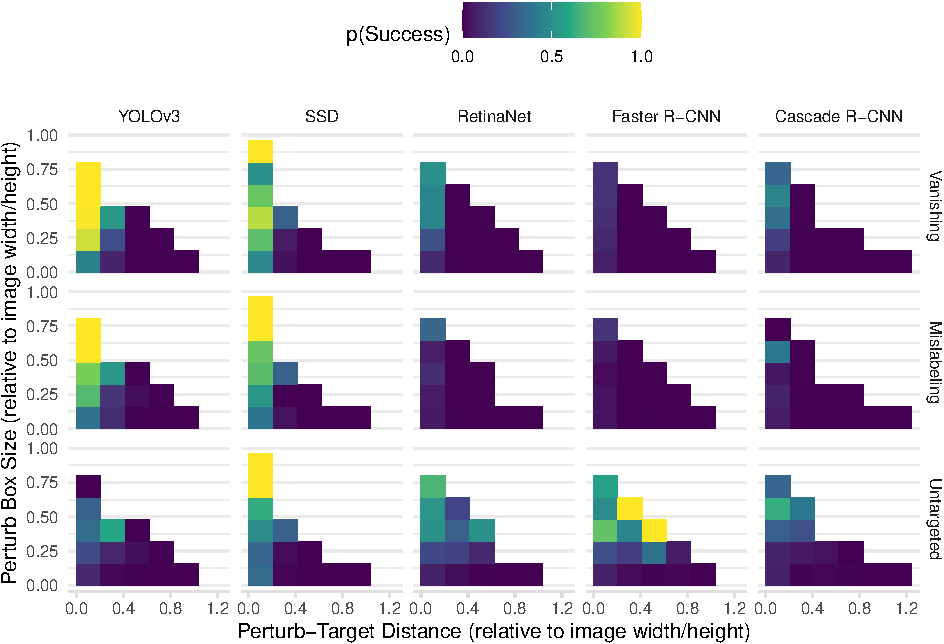
\includegraphics{imgs/perturb_bbox_and_object_dist_graph-1} 

}

\caption{Larger perturb objects significantly increase success rates for all models and attacks, except for mislabeling attack on Faster R-CNN, after controlling for perturb-target distances. Shorter perturb-target distances significantly increase success rates for all models and attacks, after controlling for perturb object sizes:  The binned summaries graph success proportion against perturb-target distance (relative to image width/height) and perturb box size (relative to image width/height) in the randomized attack experiment.}\label{fig:perturb_bbox_and_object_dist_graph}
\end{figure}

\begingroup\fontsize{9}{11}\selectfont

\begin{longtable}[t]{llllrrrrrr}
\caption{\label{tab:perturb_bbox_and_object_dist_table}We run a logistic model regressing success against perturb-target distance (relative to image width/height) and perturb box size (relative to image width/height) in the randomized attack experiment. Larger perturb objects significantly increase success rates for all models and attacks, except for mislabeling attack on Faster R-CNN, after controlling for perturb-target distances. Shorter perturb-target distances significantly increase success rates for all models and attacks, after controlling for perturb object sizes. Table headers are explained in Appendix \ref{app:tab_hdr}.}\\
\toprule
\multicolumn{2}{c}{Group} & \multicolumn{8}{c}{Regression} \\
\cmidrule(l{3pt}r{3pt}){1-2} \cmidrule(l{3pt}r{3pt}){3-10}
 & Attack & term & sig & estimate & std.error & statistic & p.value & conf.low & conf.high\\
\midrule
\addlinespace[0.3em]
\multicolumn{10}{l}{\textbf{YOLOv3}}\\
\hspace{1em} & Vanishing & distance & * & -9.672 & 0.656 & -14.738 & 0.000 & -10.986 & -8.413\\
\cmidrule{3-10}\nopagebreak
\hspace{1em} &  & size & * & 32.877 & 2.200 & 14.945 & 0.000 & 28.697 & 37.320\\
\cmidrule{3-10}\nopagebreak
\hspace{1em} &  & distance * size & * & -96.578 & 10.405 & -9.282 & 0.000 & -117.509 & -76.730\\
\cmidrule{2-10}\nopagebreak
\hspace{1em} & Mislabeling & distance & * & -8.322 & 0.516 & -16.121 & 0.000 & -9.355 & -7.331\\
\cmidrule{3-10}\nopagebreak
\hspace{1em} &  & size & * & 8.229 & 0.837 & 9.833 & 0.000 & 6.635 & 9.917\\
\cmidrule{3-10}\nopagebreak
\hspace{1em} &  & distance * size & * & -9.864 & 4.876 & -2.023 & 0.043 & -19.658 & -0.531\\
\cmidrule{2-10}\nopagebreak
\hspace{1em} & Untargeted & distance & * & -13.317 & 1.151 & -11.566 & 0.000 & -15.649 & -11.136\\
\cmidrule{3-10}\nopagebreak
\hspace{1em} &  & size & * & 1.638 & 0.647 & 2.532 & 0.011 & 0.369 & 2.909\\
\cmidrule{3-10}\nopagebreak
\hspace{1em} &  & distance * size & * & 31.584 & 5.862 & 5.388 & 0.000 & 20.028 & 43.048\\
\cmidrule{1-10}\pagebreak[0]
\addlinespace[0.3em]
\multicolumn{10}{l}{\textbf{SSD}}\\
\hspace{1em} & Vanishing & distance & * & -14.374 & 0.758 & -18.971 & 0.000 & -15.892 & -12.921\\
\cmidrule{3-10}\nopagebreak
\hspace{1em} &  & size & * & 9.330 & 0.959 & 9.729 & 0.000 & 7.508 & 11.267\\
\cmidrule{3-10}\nopagebreak
\hspace{1em} &  & distance * size &  & -7.647 & 5.626 & -1.359 & 0.174 & -18.998 & 3.079\\
\cmidrule{2-10}\nopagebreak
\hspace{1em} & Mislabeling & distance & * & -12.008 & 0.729 & -16.468 & 0.000 & -13.473 & -10.614\\
\cmidrule{3-10}\nopagebreak
\hspace{1em} &  & size & * & 7.727 & 0.806 & 9.591 & 0.000 & 6.198 & 9.357\\
\cmidrule{3-10}\nopagebreak
\hspace{1em} &  & distance * size & * & -13.614 & 5.556 & -2.451 & 0.014 & -24.820 & -3.030\\
\cmidrule{2-10}\nopagebreak
\hspace{1em} & Untargeted & distance & * & -14.125 & 0.811 & -17.425 & 0.000 & -15.757 & -12.579\\
\cmidrule{3-10}\nopagebreak
\hspace{1em} &  & size & * & 2.298 & 0.528 & 4.353 & 0.000 & 1.289 & 3.361\\
\cmidrule{3-10}\nopagebreak
\hspace{1em} &  & distance * size & * & 11.937 & 4.573 & 2.611 & 0.009 & 2.779 & 20.724\\
\cmidrule{1-10}\pagebreak[0]
\addlinespace[0.3em]
\multicolumn{10}{l}{\textbf{RetinaNet}}\\
\hspace{1em} & Vanishing & distance & * & -38.670 & 2.842 & -13.608 & 0.000 & -44.429 & -33.288\\
\cmidrule{3-10}\nopagebreak
\hspace{1em} &  & size & * & 1.917 & 0.675 & 2.840 & 0.005 & 0.647 & 3.291\\
\cmidrule{3-10}\nopagebreak
\hspace{1em} &  & distance * size & * & 53.194 & 10.742 & 4.952 & 0.000 & 31.190 & 73.157\\
\cmidrule{2-10}\nopagebreak
\hspace{1em} & Mislabeling & distance & * & -48.140 & 5.186 & -9.283 & 0.000 & -58.781 & -38.448\\
\cmidrule{3-10}\nopagebreak
\hspace{1em} &  & size & * & 2.270 & 1.151 & 1.972 & 0.049 & 0.074 & 4.594\\
\cmidrule{3-10}\nopagebreak
\hspace{1em} &  & distance * size &  & 7.234 & 25.556 & 0.283 & 0.777 & -46.376 & 53.609\\
\cmidrule{2-10}\nopagebreak
\hspace{1em} & Untargeted & distance & * & -13.171 & 1.189 & -11.082 & 0.000 & -15.598 & -10.938\\
\cmidrule{3-10}\nopagebreak
\hspace{1em} &  & size & * & 2.541 & 0.519 & 4.892 & 0.000 & 1.526 & 3.565\\
\cmidrule{3-10}\nopagebreak
\hspace{1em} &  & distance * size & * & 36.039 & 4.724 & 7.629 & 0.000 & 27.007 & 45.549\\
\cmidrule{1-10}\pagebreak[0]
\addlinespace[0.3em]
\multicolumn{10}{l}{\textbf{Faster R-CNN}}\\
\hspace{1em} & Vanishing & distance & * & -31.462 & 3.270 & -9.622 & 0.000 & -38.181 & -25.358\\
\cmidrule{3-10}\nopagebreak
\hspace{1em} &  & size & * & 3.758 & 1.086 & 3.462 & 0.001 & 1.675 & 5.942\\
\cmidrule{3-10}\nopagebreak
\hspace{1em} &  & distance * size &  & -35.320 & 23.347 & -1.513 & 0.130 & -84.636 & 7.187\\
\cmidrule{2-10}\nopagebreak
\hspace{1em} & Mislabeling & distance & * & -24.289 & 3.513 & -6.914 & 0.000 & -31.624 & -17.853\\
\cmidrule{3-10}\nopagebreak
\hspace{1em} &  & size &  & 1.648 & 1.414 & 1.166 & 0.244 & -1.207 & 4.385\\
\cmidrule{3-10}\nopagebreak
\hspace{1em} &  & distance * size &  & -37.467 & 32.660 & -1.147 & 0.251 & -108.916 & 19.888\\
\cmidrule{2-10}\nopagebreak
\hspace{1em} & Untargeted & distance & * & -14.429 & 1.244 & -11.603 & 0.000 & -16.949 & -12.074\\
\cmidrule{3-10}\nopagebreak
\hspace{1em} &  & size & * & 2.184 & 0.650 & 3.360 & 0.001 & 0.913 & 3.465\\
\cmidrule{3-10}\nopagebreak
\hspace{1em} &  & distance * size & * & 58.694 & 5.959 & 9.849 & 0.000 & 47.273 & 70.648\\
\cmidrule{1-10}\pagebreak[0]
\addlinespace[0.3em]
\multicolumn{10}{l}{\textbf{Cascade R-CNN}}\\
\hspace{1em} & Vanishing & distance & * & -27.740 & 2.837 & -9.778 & 0.000 & -33.578 & -22.453\\
\cmidrule{3-10}\nopagebreak
\hspace{1em} &  & size & * & 7.189 & 0.906 & 7.936 & 0.000 & 5.488 & 9.045\\
\cmidrule{3-10}\nopagebreak
\hspace{1em} &  & distance * size & * & -77.368 & 22.567 & -3.428 & 0.001 & -125.142 & -36.519\\
\cmidrule{2-10}\nopagebreak
\hspace{1em} & Mislabeling & distance & * & -28.681 & 3.361 & -8.533 & 0.000 & -35.680 & -22.493\\
\cmidrule{3-10}\nopagebreak
\hspace{1em} &  & size & * & 2.584 & 0.763 & 3.388 & 0.001 & 1.094 & 4.093\\
\cmidrule{3-10}\nopagebreak
\hspace{1em} &  & distance * size & * & -69.647 & 31.193 & -2.233 & 0.026 & -136.025 & -13.985\\
\cmidrule{2-10}\nopagebreak
\hspace{1em} & Untargeted & distance & * & -13.415 & 1.297 & -10.340 & 0.000 & -16.058 & -10.972\\
\cmidrule{3-10}\nopagebreak
\hspace{1em} &  & size & * & 2.594 & 0.561 & 4.621 & 0.000 & 1.492 & 3.697\\
\cmidrule{3-10}\nopagebreak
\hspace{1em} &  & distance * size & * & 25.276 & 4.976 & 5.079 & 0.000 & 15.453 & 35.061\\
\bottomrule
\end{longtable}
\endgroup{}

\begin{figure}[tb]

{\centering 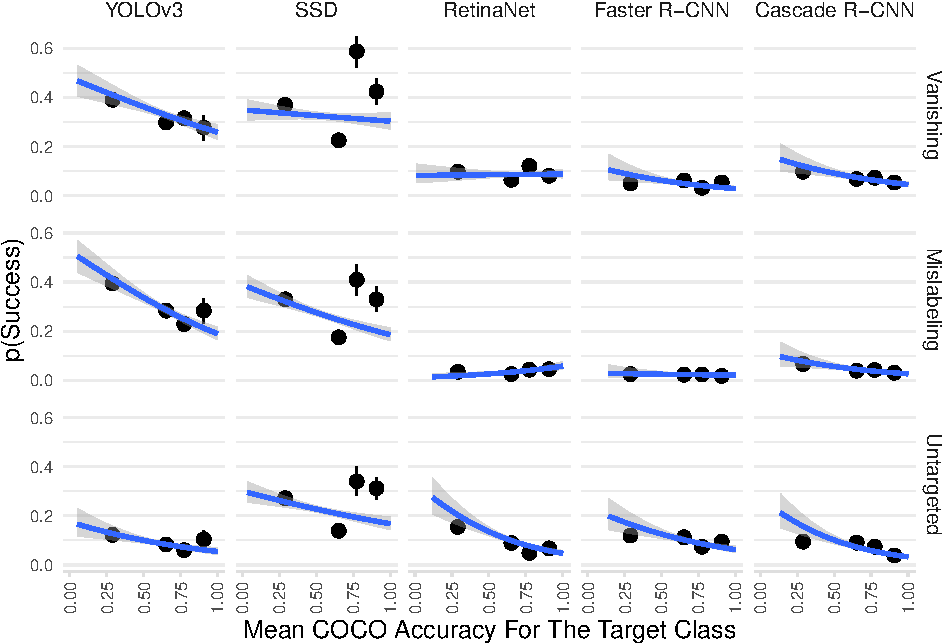
\includegraphics{imgs/target_success_graph-1} 

}

\caption{Although higher mean COCO accuracy for the target class seem to decrease success rates, the results are mixed after controlling for target class confidence (Table \ref{tab:target_success_table}):  The binned summaries and regression trendlines graph success proportion against mean COCO accuracy for the target class in the randomized attack experiment. Bins are split into quantiles. Errors are 95\% confidence intervals}\label{fig:target_success_graph}
\end{figure}

\begingroup\fontsize{9}{11}\selectfont

\begin{longtable}[t]{llllrrrrrr}
\caption{\label{tab:target_success_table}We run a logistic model regressing success against mean COCO accuracy for the target class, with target confidence as covariate, in the randomized attack experiment. The results are mixed after controlling for target class confidence and the relatively large interaction terms make interpretation challenging. Table headers are explained in Appendix \ref{app:tab_hdr}.}\\
\toprule
\multicolumn{2}{c}{Group} & \multicolumn{8}{c}{Regression} \\
\cmidrule(l{3pt}r{3pt}){1-2} \cmidrule(l{3pt}r{3pt}){3-10}
 & Attack & term & sig & estimate & std.error & statistic & p.value & conf.low & conf.high\\
\midrule
\addlinespace[0.3em]
\multicolumn{10}{l}{\textbf{YOLOv3}}\\
\hspace{1em} & Vanishing & accuracy &  & 0.726 & 0.732 & 0.992 & 0.321 & -0.707 & 2.164\\
\cmidrule{3-10}\nopagebreak
\hspace{1em} &  & confidence &  & 0.733 & 0.652 & 1.124 & 0.261 & -0.544 & 2.014\\
\cmidrule{3-10}\nopagebreak
\hspace{1em} &  & accuracy * confidence & * & -2.196 & 0.976 & -2.250 & 0.024 & -4.113 & -0.285\\
\cmidrule{2-10}\nopagebreak
\hspace{1em} & Mislabeling & accuracy &  & 1.133 & 0.743 & 1.524 & 0.128 & -0.325 & 2.591\\
\cmidrule{3-10}\nopagebreak
\hspace{1em} &  & confidence &  & 0.044 & 0.679 & 0.065 & 0.948 & -1.289 & 1.373\\
\cmidrule{3-10}\nopagebreak
\hspace{1em} &  & accuracy * confidence & * & -3.371 & 1.025 & -3.289 & 0.001 & -5.382 & -1.363\\
\cmidrule{2-10}\nopagebreak
\hspace{1em} & Untargeted & accuracy &  & 1.324 & 1.060 & 1.248 & 0.212 & -0.749 & 3.410\\
\cmidrule{3-10}\nopagebreak
\hspace{1em} &  & confidence &  & -1.696 & 1.113 & -1.525 & 0.127 & -3.895 & 0.469\\
\cmidrule{3-10}\nopagebreak
\hspace{1em} &  & accuracy * confidence & * & -3.376 & 1.697 & -1.989 & 0.047 & -6.701 & -0.047\\
\cmidrule{1-10}\pagebreak[0]
\addlinespace[0.3em]
\multicolumn{10}{l}{\textbf{SSD}}\\
\hspace{1em} & Vanishing & accuracy & * & 1.282 & 0.511 & 2.508 & 0.012 & 0.283 & 2.288\\
\cmidrule{3-10}\nopagebreak
\hspace{1em} &  & confidence &  & 0.017 & 0.426 & 0.040 & 0.968 & -0.816 & 0.854\\
\cmidrule{3-10}\nopagebreak
\hspace{1em} &  & accuracy * confidence & * & -1.907 & 0.710 & -2.684 & 0.007 & -3.304 & -0.519\\
\cmidrule{2-10}\nopagebreak
\hspace{1em} & Mislabeling & accuracy & * & 3.281 & 0.549 & 5.976 & 0.000 & 2.210 & 4.363\\
\cmidrule{3-10}\nopagebreak
\hspace{1em} &  & confidence & * & 1.871 & 0.460 & 4.067 & 0.000 & 0.972 & 2.776\\
\cmidrule{3-10}\nopagebreak
\hspace{1em} &  & accuracy * confidence & * & -6.178 & 0.795 & -7.769 & 0.000 & -7.747 & -4.629\\
\cmidrule{2-10}\nopagebreak
\hspace{1em} & Untargeted & accuracy & * & 4.517 & 0.584 & 7.738 & 0.000 & 3.381 & 5.670\\
\cmidrule{3-10}\nopagebreak
\hspace{1em} &  & confidence & * & 1.990 & 0.499 & 3.985 & 0.000 & 1.014 & 2.971\\
\cmidrule{3-10}\nopagebreak
\hspace{1em} &  & accuracy * confidence & * & -7.783 & 0.874 & -8.905 & 0.000 & -9.508 & -6.081\\
\cmidrule{1-10}\pagebreak[0]
\addlinespace[0.3em]
\multicolumn{10}{l}{\textbf{RetinaNet}}\\
\hspace{1em} & Vanishing & accuracy &  & 1.009 & 1.143 & 0.883 & 0.377 & -1.217 & 3.262\\
\cmidrule{3-10}\nopagebreak
\hspace{1em} &  & confidence & * & -3.823 & 1.744 & -2.192 & 0.028 & -7.277 & -0.442\\
\cmidrule{3-10}\nopagebreak
\hspace{1em} &  & accuracy * confidence &  & 0.571 & 2.246 & 0.254 & 0.799 & -3.819 & 4.984\\
\cmidrule{2-10}\nopagebreak
\hspace{1em} & Mislabeling & accuracy &  & 2.565 & 2.044 & 1.255 & 0.209 & -1.385 & 6.612\\
\cmidrule{3-10}\nopagebreak
\hspace{1em} &  & confidence & * & -8.994 & 3.794 & -2.371 & 0.018 & -16.549 & -1.716\\
\cmidrule{3-10}\nopagebreak
\hspace{1em} &  & accuracy * confidence &  & 2.506 & 4.691 & 0.534 & 0.593 & -6.650 & 11.687\\
\cmidrule{2-10}\nopagebreak
\hspace{1em} & Untargeted & accuracy & * & 2.471 & 1.206 & 2.049 & 0.040 & 0.109 & 4.837\\
\cmidrule{3-10}\nopagebreak
\hspace{1em} &  & confidence &  & -1.214 & 1.810 & -0.671 & 0.503 & -4.820 & 2.279\\
\cmidrule{3-10}\nopagebreak
\hspace{1em} &  & accuracy * confidence & * & -6.672 & 2.553 & -2.613 & 0.009 & -11.666 & -1.654\\
\cmidrule{1-10}\pagebreak[0]
\addlinespace[0.3em]
\multicolumn{10}{l}{\textbf{Faster R-CNN}}\\
\hspace{1em} & Vanishing & accuracy & * & -5.572 & 1.544 & -3.608 & 0.000 & -8.586 & -2.520\\
\cmidrule{3-10}\nopagebreak
\hspace{1em} &  & confidence & * & -6.548 & 1.557 & -4.206 & 0.000 & -9.623 & -3.513\\
\cmidrule{3-10}\nopagebreak
\hspace{1em} &  & accuracy * confidence & * & 6.505 & 2.134 & 3.047 & 0.002 & 2.327 & 10.700\\
\cmidrule{2-10}\nopagebreak
\hspace{1em} & Mislabeling & accuracy &  & -4.008 & 2.072 & -1.935 & 0.053 & -7.990 & 0.140\\
\cmidrule{3-10}\nopagebreak
\hspace{1em} &  & confidence & * & -10.366 & 2.631 & -3.940 & 0.000 & -15.562 & -5.263\\
\cmidrule{3-10}\nopagebreak
\hspace{1em} &  & accuracy * confidence & * & 8.374 & 3.358 & 2.494 & 0.013 & 1.781 & 14.920\\
\cmidrule{2-10}\nopagebreak
\hspace{1em} & Untargeted & accuracy & * & -3.045 & 1.151 & -2.646 & 0.008 & -5.305 & -0.788\\
\cmidrule{3-10}\nopagebreak
\hspace{1em} &  & confidence & * & -6.522 & 1.247 & -5.229 & 0.000 & -8.997 & -4.105\\
\cmidrule{3-10}\nopagebreak
\hspace{1em} &  & accuracy * confidence & * & 3.928 & 1.670 & 2.353 & 0.019 & 0.676 & 7.222\\
\cmidrule{1-10}\pagebreak[0]
\addlinespace[0.3em]
\multicolumn{10}{l}{\textbf{Cascade R-CNN}}\\
\hspace{1em} & Vanishing & accuracy & * & -3.474 & 1.409 & -2.466 & 0.014 & -6.223 & -0.691\\
\cmidrule{3-10}\nopagebreak
\hspace{1em} &  & confidence & * & -3.241 & 1.281 & -2.530 & 0.011 & -5.742 & -0.712\\
\cmidrule{3-10}\nopagebreak
\hspace{1em} &  & accuracy * confidence &  & 3.012 & 1.787 & 1.685 & 0.092 & -0.505 & 6.509\\
\cmidrule{2-10}\nopagebreak
\hspace{1em} & Mislabeling & accuracy &  & -2.849 & 1.600 & -1.780 & 0.075 & -5.961 & 0.326\\
\cmidrule{3-10}\nopagebreak
\hspace{1em} &  & confidence & * & -4.204 & 1.580 & -2.661 & 0.008 & -7.303 & -1.099\\
\cmidrule{3-10}\nopagebreak
\hspace{1em} &  & accuracy * confidence &  & 2.670 & 2.171 & 1.229 & 0.219 & -1.600 & 6.920\\
\cmidrule{2-10}\nopagebreak
\hspace{1em} & Untargeted & accuracy &  & -0.996 & 1.283 & -0.776 & 0.438 & -3.504 & 1.532\\
\cmidrule{3-10}\nopagebreak
\hspace{1em} &  & confidence &  & -2.287 & 1.256 & -1.821 & 0.069 & -4.759 & 0.171\\
\cmidrule{3-10}\nopagebreak
\hspace{1em} &  & accuracy * confidence &  & -1.014 & 1.751 & -0.579 & 0.562 & -4.446 & 2.423\\
\bottomrule
\end{longtable}
\endgroup{}

\begin{figure}[tb]

{\centering 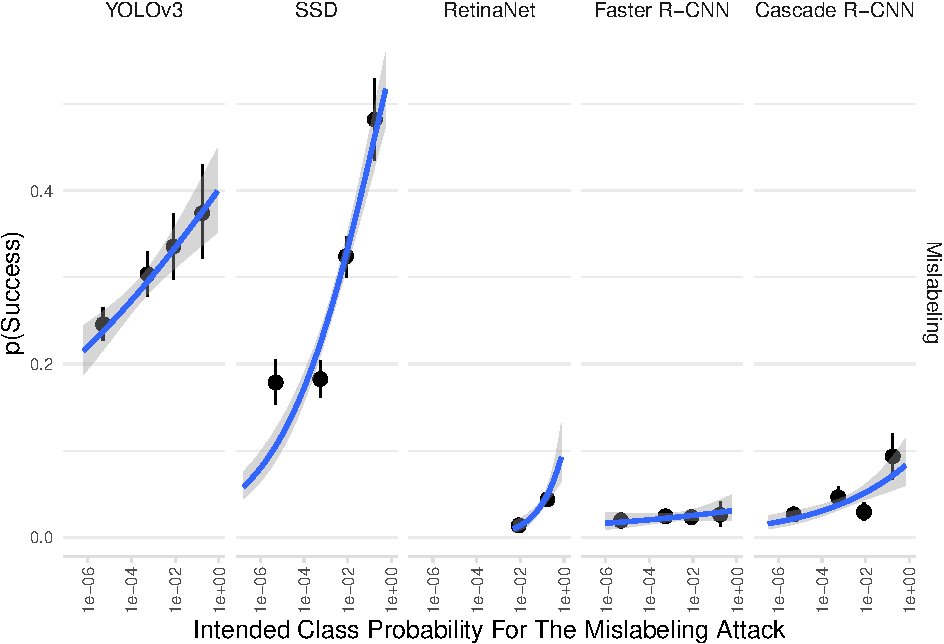
\includegraphics{imgs/mislabel_conf_graph-1} 

}

\caption{Although intended class probability seem to increase success rates for the mislabeling attack, it does not predict success rates after controlling for target class confidence, except for RetinaNet (Table \ref{tab:mislabel_conf_table}):  The binned summaries and regression trendlines graph success proportion against intended class probability in the randomized attack experiment. Bins are split into quantiles. Errors are 95\% confidence intervals}\label{fig:mislabel_conf_graph}
\end{figure}

\begingroup\fontsize{9}{11}\selectfont

\begin{longtable}[t]{llllrrrrrr}
\caption{\label{tab:mislabel_conf_table}We run a logistic model regressing success against log(intended class probability) for the mislabeling attack, with predicted class's confidence as covariate, in the randomized attack experiment. Intended class probability does not predict success rates after controlling for target class confidence, except for RetinaNet. Table headers are explained in Appendix \ref{app:tab_hdr}.}\\
\toprule
\multicolumn{2}{c}{Group} & \multicolumn{8}{c}{Regression} \\
\cmidrule(l{3pt}r{3pt}){1-2} \cmidrule(l{3pt}r{3pt}){3-10}
 & Model & term & sig & estimate & std.error & statistic & p.value & conf.low & conf.high\\
\midrule
\addlinespace[0.3em]
\multicolumn{10}{l}{\textbf{Mislabeling}}\\
\hspace{1em} & YOLOv3 & log(probability) & * & -0.202 & 0.040 & -5.028 & 0.000 & -0.281 & -0.123\\
\cmidrule{3-10}\nopagebreak
\hspace{1em} &  & confidence &  & 0.758 & 0.485 & 1.563 & 0.118 & -0.192 & 1.712\\
\cmidrule{3-10}\nopagebreak
\hspace{1em} &  & log(probability) * confidence & * & 0.363 & 0.057 & 6.337 & 0.000 & 0.251 & 0.476\\
\cmidrule{2-10}\nopagebreak
\hspace{1em} & SSD & log(probability) &  & 0.058 & 0.047 & 1.242 & 0.214 & -0.033 & 0.150\\
\cmidrule{3-10}\nopagebreak
\hspace{1em} &  & confidence &  & -0.161 & 0.429 & -0.375 & 0.707 & -1.001 & 0.682\\
\cmidrule{3-10}\nopagebreak
\hspace{1em} &  & log(probability) * confidence & * & 0.144 & 0.064 & 2.264 & 0.024 & 0.020 & 0.270\\
\cmidrule{2-10}\nopagebreak
\hspace{1em} & RetinaNet & log(probability) & * & 0.683 & 0.325 & 2.101 & 0.036 & 0.036 & 1.308\\
\cmidrule{3-10}\nopagebreak
\hspace{1em} &  & confidence & * & -8.137 & 1.846 & -4.408 & 0.000 & -11.802 & -4.567\\
\cmidrule{3-10}\nopagebreak
\hspace{1em} &  & log(probability) * confidence &  & -0.842 & 0.703 & -1.198 & 0.231 & -2.183 & 0.571\\
\cmidrule{2-10}\nopagebreak
\hspace{1em} & Faster R-CNN & log(probability) &  & 0.018 & 0.115 & 0.156 & 0.876 & -0.209 & 0.242\\
\cmidrule{3-10}\nopagebreak
\hspace{1em} &  & confidence & * & -5.405 & 1.292 & -4.183 & 0.000 & -7.955 & -2.880\\
\cmidrule{3-10}\nopagebreak
\hspace{1em} &  & log(probability) * confidence &  & -0.165 & 0.167 & -0.987 & 0.324 & -0.489 & 0.167\\
\cmidrule{2-10}\nopagebreak
\hspace{1em} & Cascade R-CNN & log(probability) &  & -0.022 & 0.095 & -0.237 & 0.813 & -0.210 & 0.162\\
\cmidrule{3-10}\nopagebreak
\hspace{1em} &  & confidence &  & -1.592 & 0.871 & -1.827 & 0.068 & -3.282 & 0.139\\
\cmidrule{3-10}\nopagebreak
\hspace{1em} &  & log(probability) * confidence &  & 0.094 & 0.124 & 0.756 & 0.450 & -0.146 & 0.340\\
\bottomrule
\end{longtable}
\endgroup{}

\begin{figure}[tb]

{\centering 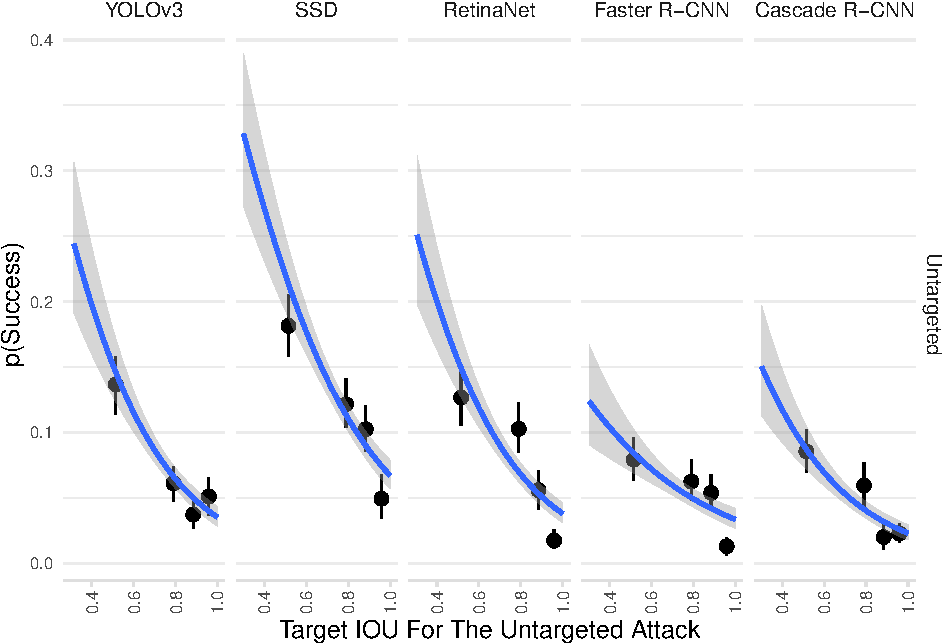
\includegraphics{imgs/untarget_iou_graph-1} 

}

\caption{Target IOU for the untargeted attack increases success rates on all models:  The binned summaries and regression trendlines graph success proportion against target IOU for the untargeted attack in the randomized attack experiment. Bins are split into quantiles. Errors are 95\% confidence intervals}\label{fig:untarget_iou_graph}
\end{figure}

\begingroup\fontsize{9}{11}\selectfont

\begin{longtable}[t]{llllrrrrrr}
\caption{\label{tab:untarget_iou_table}We run a logistic model regressing success against target IOU for the untargeted attack in the randomized attack experiment. Target IOU for the untargeted attack increases success rates on all models. Table headers are explained in Appendix \ref{app:tab_hdr}.}\\
\toprule
\multicolumn{2}{c}{Group} & \multicolumn{8}{c}{Regression} \\
\cmidrule(l{3pt}r{3pt}){1-2} \cmidrule(l{3pt}r{3pt}){3-10}
 & Model & term & sig & estimate & std.error & statistic & p.value & conf.low & conf.high\\
\midrule
\addlinespace[0.3em]
\multicolumn{10}{l}{\textbf{Untargeted}}\\
\hspace{1em} & YOLOv3 & bbox\_iou\_eval & * & -2.526 & 0.341 & -7.417 & 0 & -3.189 & -1.853\\
\cmidrule{2-10}\nopagebreak
\hspace{1em} & SSD & bbox\_iou\_eval & * & -3.254 & 0.235 & -13.838 & 0 & -3.716 & -2.794\\
\cmidrule{2-10}\nopagebreak
\hspace{1em} & RetinaNet & bbox\_iou\_eval & * & -2.130 & 0.308 & -6.904 & 0 & -2.730 & -1.520\\
\cmidrule{2-10}\nopagebreak
\hspace{1em} & Faster R-CNN & bbox\_iou\_eval & * & -1.899 & 0.294 & -6.460 & 0 & -2.471 & -1.318\\
\cmidrule{2-10}\nopagebreak
\hspace{1em} & Cascade R-CNN & bbox\_iou\_eval & * & -2.566 & 0.318 & -8.062 & 0 & -3.187 & -1.938\\
\bottomrule
\end{longtable}
\endgroup{}

\end{document}
